
% Operator
\usepackage{xspace}

\newcommand{\ident}[2]{\newcommand{#1}{\ensuremath{\mathrm{#2}\xspace}}}
\newcommand{\operator}[2]{\newcommand{#1}{\ensuremath{\mathop{#2}\xspace}}}

% Domain

\newcommand{\defDom}[2]{\newcommand{#1}{\ensuremath{\mathbb {#2}}}\xspace}

\defDom{\N}{N}
\defDom{\Z}{Z}
\defDom{\Q}{Q}
\defDom{\R}{R}
\defDom{\C}{C}
\defDom{\Pri}{P}
\defDom{\D}{D}

\newcommand{\prom}[1]{\ensuremath{\widehat{{#1}^\ast}}\xspace}

\newcommand{\aut}[1]{\ensuremath{\mathcal {#1}}\xspace}

% Borel and analytic sets

\newcommand{\boldclass}[3]{\ensuremath{\mathbf{#1}^{#2}_{#3}}}
\newcommand{\lightclass}[3]{\ensuremath{{#1}^{#2}_{#3}}}

\newcommand{\borel}{\ensuremath{\mathcal B}\xspace}

\newcommand{\bsigma}[1]{\boldclass{\Sigma}{0}{#1}}
\newcommand{\bpi}[1]{\boldclass{\Pi}{0}{#1}}
\newcommand{\bdelta}[1]{\boldclass{\Delta}{0}{#1}}

\newcommand{\asigma}[1]{\boldclass{\Sigma}{1}{#1}}
\newcommand{\api}[1]{\boldclass{\Pi}{1}{#1}}
\newcommand{\adelta}[1]{\boldclass{\Delta}{1}{#1}}

\newcommand{\esigma}[2]{\lightclass{\Sigma}{#1}{#2}}
\newcommand{\epi}[2]{\lightclass{\Pi}{1}{#1}}
\newcommand{\edelta}[2]{\lightclass{\Delta}{#1}{#2}}

\newcommand{\bc}[1]{\mathcal{BC}({#1})}

\newcommand{\mathnm}[1]{#1}
\newcommand{\lex}{<_{\mathrm{\mathnm{lex}}}}
\newcommand{\lexeq}{\leq_{\mathrm{\mathnm{lex}}}}

\newcommand{\wadge}{<_{\mathrm{\mathnm{W}}}}
\newcommand{\wadgeq}{\leq_{\mathrm{\mathnm{W}}}}

\newcommand{\mathcalsym}[1]{\ensuremath{\mathcal{#1}}\xspace}


\newcommand{\Aa}{\mathcalsym{A}}
\newcommand{\Bb}{\mathcalsym{B}}
\newcommand{\Cc}{\mathcalsym{C}}
\newcommand{\Dd}{\mathcalsym{D}}
\newcommand{\Ee}{\mathcalsym{E}}
\newcommand{\Ff}{\mathcalsym{F}}
\newcommand{\Gg}{\mathcalsym{G}}
\newcommand{\Hh}{\mathcalsym{H}}
\newcommand{\Ii}{\mathcalsym{I}}
\newcommand{\Jj}{\mathcalsym{J}}
\newcommand{\Kk}{\mathcalsym{K}}
\newcommand{\Ll}{\mathcalsym{L}}
\newcommand{\Mm}{\mathcalsym{M}}
\newcommand{\Nn}{\mathcalsym{N}}
\newcommand{\Oo}{\mathcalsym{O}}
\newcommand{\Pl}{\mathcalsym{P}}
\newcommand{\Ql}{\mathcalsym{Q}}
\newcommand{\Rr}{\mathcalsym{R}}
\newcommand{\Ss}{\mathcalsym{S}}
\newcommand{\Tt}{\mathcalsym{T}}
\newcommand{\Uu}{\mathcalsym{U}}
\newcommand{\Vv}{\mathcalsym{V}}
\newcommand{\Ww}{\mathcalsym{W}}
\newcommand{\Xx}{\mathcalsym{X}}
\newcommand{\Yy}{\mathcalsym{Y}}
\newcommand{\Zz}{\mathcalsym{Z}}


% Comment

% Functions

\newcommand{\fun}[3]{\ensuremath{#1\colon #2 \to #3}}
\newcommand{\parfun}[3]{\ensuremath{#1\colon #2 \rightharpoonup #3}}

\ident{\dom}{dom}
\ident{\rg}{rg}
\ident{\id}{id}
\ident{\sgn}{sgn}

\ident{\prof}{Profiles}

\ident{\type}{tp}
\ident{\types}{Tp}

\ident{\errTrace}{NotTrace}
\ident{\errProfile}{NoProfile}

% Operations

\ident{\close}{cl}
\ident{\inter}{int}
\ident{\lang}{L}

\newcommand{\restr}{\!\upharpoonright}

\newcommand{\newton}[2]{\ensuremath{\binom{#1}{#2}}}

\newcommand{\comp}[1]{\ensuremath{\overline{#1}}}

% Hierarchies

\newcommand{\bhiers}{
\begin{center}
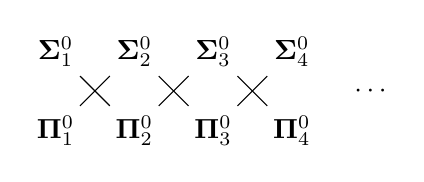
\begin{tikzpicture}
  \foreach \x in {1, 2, 3, 4} {
    \node (s-\x) at (\x,0.5) {$\bsigma{\x}$};
    \node (p-\x) at (\x,-0.5) {$\bpi{\x}$};
  }

  \node at (5,0) {$\cdots$};

  \foreach \from/\to in {1/2, 2/3, 3/4} {
    \draw[-] (p-\from) -- (s-\to);
    \draw[-] (s-\from) -- (p-\to);
  }

\end{tikzpicture}
\end{center}
}

\newcommand{\bhier}{
\begin{center}
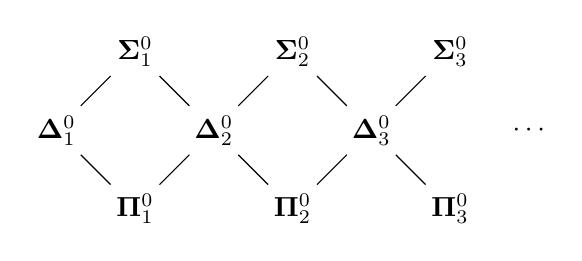
\begin{tikzpicture}
  \newcommand{\w}{2}
  \foreach \x in {1, 2, 3} {
    \node (s-\x) at (\w*\x-1,1) {$\bsigma{\x}$};
    \node (p-\x) at (\w*\x-1,-1) {$\bpi{\x}$};
  }

  \foreach \x in {1, 2, 3} {
    \node (d-\x) at (\w*\x-2,0) {$\bdelta{\x}$};
  }

  \node at (\w*3,0) {$\cdots$};

  \foreach \from/\to in {1/2, 2/3} {
    \draw[-] (p-\from) -- (d-\from);
    \draw[-] (s-\from) -- (d-\from);

    \draw[-] (d-\to) -- (p-\from);
    \draw[-] (d-\to) -- (s-\from);
  }

  \draw[-] (d-3) -- (s-3);
  \draw[-] (d-3) -- (p-3);

\end{tikzpicture}
\end{center}
}

\newcommand{\bhiere}{
\begin{center}
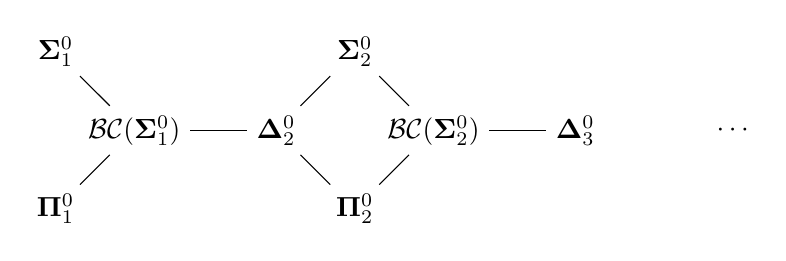
\begin{tikzpicture}
  \newcommand{\w}{3.8}
  \foreach \x in {1, 2} {
    \node (s-\x) at (\w*\x-1,1) {$\bsigma{\x}$};
    \node (b-\x) at (\w*\x,0) {$\bc{\bsigma{\x}}$};
    \node (p-\x) at (\w*\x-1,-1) {$\bpi{\x}$};
  }

  \foreach \x in {2, 3} {
    \node (d-\x) at (\w*\x-2,0) {$\bdelta{\x}$};
  }

  \node at (\w*3,0) {$\cdots$};

  \foreach \from/\to in {1/2, 2/3} {
    \draw[-] (p-\from) -- (b-\from);
    \draw[-] (s-\from) -- (b-\from);

    \draw[-] (b-\from) -- (d-\to);
  }

  \draw[-] (d-2) -- (s-2);
  \draw[-] (d-2) -- (p-2);

\end{tikzpicture}
\end{center}
}


\newcommand{\ahiers}{
\begin{center}
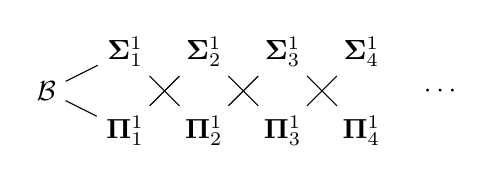
\begin{tikzpicture}
  \node (b) at (0,0) {$\borel$};

  \foreach \x in {1, 2, 3, 4} {
    \node (s-\x) at (\x,0.5) {$\asigma{\x}$};
    \node (p-\x) at (\x,-0.5) {$\api{\x}$};
  }

  \node at (5,0) {$\cdots$};

  \foreach \from/\to in {1/2, 2/3, 3/4} {
    \draw (p-\from) -- (s-\to);
    \draw (s-\from) -- (p-\to);
  }

  \draw (b) -- (p-1);
  \draw (b) -- (s-1);

\end{tikzpicture}
\end{center}
}


\newcommand{\ahiere}{
\begin{center}
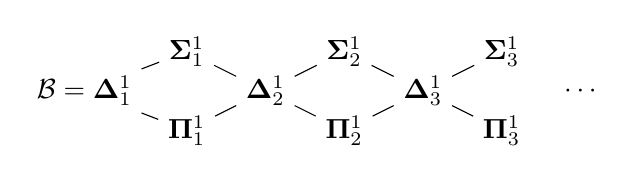
\begin{tikzpicture}
  \node (d-1) at (0.7,0) {$\borel=\adelta{1}$};

  \foreach \x in {1, 2, 3} {
    \node (s-\x) at (2*\x, 0.5) {$\asigma{\x}$};
    \node (p-\x) at (2*\x,-0.5) {$\api{\x}$};
  }

  \foreach \x in {2, 3} {
    \node (d-\x) at (2*\x-1,0) {$\adelta{\x}$};
  }

  \node at (2*3+1,0) {$\cdots$};

  \foreach \from/\to in {1/2, 2/3} {
    \draw (p-\from) -- (d-\to);
    \draw (s-\from) -- (d-\to);
    \draw (d-\to) -- (s-\to);
    \draw (d-\to) -- (p-\to);
  }

  \draw (d-1) -- (p-1);
  \draw (d-1) -- (s-1);

\end{tikzpicture}
\end{center}
}


\newcommand{\hiers}{
\begin{center}
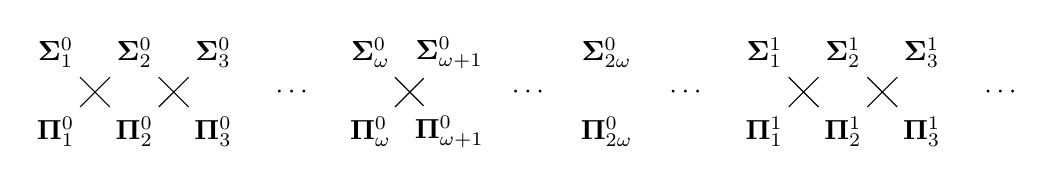
\begin{tikzpicture}
  \foreach \x in {1, 2, 3} {
    \node (s-\x) at (\x-6,0.5) {$\bsigma{\x}$};
    \node (p-\x) at (\x-6,-0.5) {$\bpi{\x}$};
  }

  \foreach \from/\to in {1/2, 2/3} {
    \draw[-] (p-\from) -- (s-\to);
    \draw[-] (s-\from) -- (p-\to);
  }

  \node at (-2,0) {$\cdots$};

  \node (so-0) at (-1,0.5) {$\bsigma{\omega}$};
  \node (po-0) at (-1,-0.5) {$\bpi{\omega}$};

  \node (so-1) at (0,0.5) {$\bsigma{\omega+1}$};
  \node (po-1) at (0,-0.5) {$\bpi{\omega+1}$};

  \draw (po-0) -- (so-1);
  \draw (so-0) -- (po-1);

  \node at (1,0) {$\cdots$};

  \node (s2o-1) at (2,0.5) {$\bsigma{2\omega}$};
  \node (p2o-1) at (2,-0.5) {$\bpi{2\omega}$};

  \node at (3,0) {$\cdots$};

  \foreach \x in {1, 2, 3} {
    \node (s-\x) at (\x+3,0.5) {$\asigma{\x}$};
    \node (p-\x) at (\x+3,-0.5) {$\api{\x}$};
  }

  \node at (4+3,0) {$\cdots$};

  \foreach \from/\to in {1/2, 2/3} {
    \draw (p-\from) -- (s-\to);
    \draw (s-\from) -- (p-\to);
  }
\end{tikzpicture}
\end{center}
}


% MACROS =======================================================================

\ident{\BC}{BC}

% the space of trees over a given alphabet
\newcommand{\trees}[1]{\ensuremath{\mathrm{Tr}_{{#1}}}\xspace}

% the space of partial trees over a given alphabet
\newcommand{\partrees}[1]{\ensuremath{\mathrm{PTr}_{{#1}}}\xspace}

\ident{\holes}{holes}

\ident{\graph}{Gph}

\ident{\cmp}{Comp}

% the first (positive) player Eve
\newcommand{\eve}{\ensuremath{\exists}\xspace}

% the second (negative) player Adam
\newcommand{\adam}{\ensuremath{\forall}\xspace}

% Eves move
\newcommand{\tranE}[1]{\ensuremath{\left<{#1}\right>}\xspace}

% Adams move
\newcommand{\tranA}[1]{\ensuremath{\left[{#1}\right]}\xspace}

% HIERARCHIES ==================================================================

% language W like Walukiewicz
\newcommand{\W}[2]{\ensuremath{W_{{#1},{#2}}}\xspace}

% the Rabin-Mostowski hierarchy
\ident{\RM}{RM}

\ident{\RMD}{RM\Delta}

\newcommand{\RModd}[1]{\ensuremath{\mathbf{\Sigma}^{RM}_{#1}}\xspace}
\newcommand{\RMeven}[1]{\ensuremath{\mathbf{\Pi}^{RM}_{#1}}\xspace}
\newcommand{\RMdelta}[1]{\ensuremath{\mathbf{\Delta}^{RM}_{#1}}\xspace}

% the topological index hierarchy
\newcommand{\Wsigma}[1]{\ensuremath{\mathbf{\Sigma}^W_{#1}}\xspace}
\newcommand{\Wpi}[1]{\ensuremath{\mathbf{\Pi}^W_{#1}}\xspace}
\newcommand{\Wdelta}[1]{\ensuremath{\mathbf{\Delta}^W_{#1}}\xspace}

% INDICES =======================================================================

% some rank
\newcommand{\rank}{r}

% lowest rank in flower
\newcommand{\rmin}{i}

% highest rank in flower
\newcommand{\rmax}{j}

\ident{\br}{Branching}

% INDUCTION ========================================================================

\ident{\level}{level}

\ident{\class}{class}

\ident{\hlev}{RMlev}

%\newcommand{\tran}[1]{\overset{#1}{\longrightarrow}}
\newcommand{\tran}[1]{\xrightarrow{#1}}


\ident{\game}{\mathbf{G}}


% games for alternating automata
\ident{\agame}{{\mathbf{G}}}

%games for game automata - associated with runs
\ident{\rhogame}{{\mathbf{G_\rho}}}

\newcommand{\hole}{\Box}

%Comments
\newcommand{\boxcomment}[1]{
\begin{center}\fbox{\parbox{8.6cm}{#1}}\end{center}}

\newcommand{\ale}[1]{\boxcomment{{\bf Alessandro: } #1}}
\newcommand{\filip}[1]{\boxcomment{{\bf Filip: }#1}}
\newcommand{\michal}[1]{\boxcomment{{\bf Micha\l: }#1}}


% Theorems and lemmas in the appendix. 
\newcommand\thmheadfont{\upshape\bf}
\newenvironment{thmapp}[1]{\noindent {\thmheadfont #1}.\ \itshape }
{\smallskip}

%% replaced A-simulations with \herewasA simulations, can revert it,
%% it someone defends it. I can see no point in it, since there are no
%% T-simulations any more.

\newcommand{\herewasA}{}


\renewcommand{\setminus}{-}

\newcommand{\init}{I}

\newcommand{\dt}{\mathrm{det}}


\newcommand{\dL}{\mathtt{L}}
\newcommand{\dR}{\mathtt{R}}

\ident{\weak}{\mathit{w}}

\ident{\wclass}{wclass}

% games for alternating automata
%\ident{\agame}{{\mathbf{G}}}

%games for game automata - associated with runs
%\ident{\rhogame}{{\mathbf{G_\rho}}}

%\ident{\holes}{holes}
\ident{\leave}{\textit{leave}}
\ident{\stay}{\textit{stay}}

\newcommand{\wRMeven}[1]{\ensuremath{\mathbf{\Pi}^{\weak}_{#1}}\xspace}
\newcommand{\wRModd}[1]{\ensuremath{\mathbf{\Sigma}^{\weak}_{#1}}\xspace}
\newcommand{\wRMdelta}[1]{\ensuremath{\mathbf{\Delta}^{\!\weak}_{#1}}\xspace}

\newcommand{\wRM}{\textrm{\bf{RM}}^{\weak}}

\newcommand{\edel}[8]{
  \node (p)  [] at (#1+0,0) {$p$};
  \node (e)  [] at (#1-1.5,1) {$q^{#2}$};  
  \node (a)  [] at (#1+1.5,1) {$q^{#3}$};     
  \node (el) [] at (#1-2.6,0.6) {$q^{#2}_L$};  
  \node (er) [] at (#1-1.5,2.15) {$q^{#2}_R$};  
  \node (al) [] at (#1+1.5,2.15) {$q^{#3}_L$};   
  \node (ar) [] at (#1+2.6,0.6) {$q^{#3}_R$};

  \node at (#1-1.5,0.3) {$#6$};
  \node at (#1-0.8,1.2) {$#7$};
  \node at (#1+0.8,1.2) {$#7$};
  \node at (#1+1.5,0.3) {$#8$};
  
  \path[->]
    (p) edge[in=-80, out=-30, looseness=0.8, loop, distance=2cm] node[above left] {$#4$} (p)
    (p) edge[in=-100, out=210, looseness=0.8, loop, distance=2cm] node[above right] {$#5$} (p)
    (p) edge node {} (e)
    (e) edge[out=150, in=75] node {} (el)
    (e) edge[out=150, in=215] node {} (er)
    (p) edge node {} (a)
    (a) edge[out=30, in=-35] node {} (al)
    (a) edge[out=30, in=105] node {} (ar)
    (al) edge[bend right] node {} (p)
    (ar) edge[bend left] node {} (p)
    (el) edge[bend right] node {} (p)
    (er) edge[bend left] node {} (p);   
}

\newcommand{\figEdelNew}{
\begin{figure}
\centering
\begin{tikzpicture}[->,>=stealth',scale=0.85, every node/.style={scale=0.77}]
\edel{-4}{\eve}{\adam}01234
\edel{ 4}{\adam}{\eve}12345
\end{tikzpicture}
%\vspace{-7ex}
\caption{$(0,4)$-edelweiss and $(1,5)$-edelweiss.}
\label{fig:edelweiss}
%\vspace{-4ex}
\end{figure}
}